\section{The Existence and Uniqueness Theorem}
    Consider the initial value problem
    \begin{equation*}
        y' = f(t, y), \qquad y(0) = 0
    \end{equation*}
    If an initial value problem is not of this form, we can apply a translation of the coordinate axes that will take $(t_0, y_0)$ to the origin.
    \begin{theorem}
        If $f$ and $\pdv{f}{y}$ are continuous in a rectangle $R: |t| \leq a, |y| \leq b$, then there is some interval $|t| \leq h \leq a$ in which there exists a unique solution $y = \phi(t)$ of the initial value problem.
    \end{theorem}
    If we integrate the initial value problem equation, we get
    \begin{equation*}
        \phi(t) = \int_0^t f[s, \phi(s)] ds
    \end{equation*}
    This is called the \textbf{integral equation}, which is equivalent to the initial value equation.
    \newline \indent
    One method of showing that the integral equation has a unique solution is the \textbf{method of successive approximations} or Picard's \textbf{iteration method}. In using this method, we start by choosing an initial function $\phi_0$, either arbitrarily or to approximate the solution. The simplest choice is $$\phi_0(t) = 0$$ $\phi_0$ satisfies the initial condition, but probably not the differential equation. The next apprximation $\phi_1$ is obtained using $\phi_0$.
    \begin{equation*}
        \phi_1(t) = \int_0^t f[s, \phi_0(s)] ds
    \end{equation*}
    and, in general,
    \begin{equation*}
        \phi_{n+1}(t) = \int_0^t f[s, \phi_n(s)] ds
    \end{equation*}
    This creates a sequence of functions ${\phi_n}= {\phi_0, \phi_1, \phi_2, \dots, \phi_n, \dots}$. Each element of the sequence satisfies the initial condition, but in general none satisfies the differential equation. If at some stage $\phi_{k+1}(t) = \phi_k(t)$, then it follows that $\phi_k$ is a solution and does follow the differential equation.
    \begin{enumerate}
        \item \textbf{Do all members of the sequence ${\phi_n}$ exist?}
            \newline \indent
            If $f$ and $\pdv{f}{y}$ are continuous in the whole $ty$-plane, then each $\phi_n$ is known to exist and can be calculated. But if $f$ and $\pdv{f}{y}$ are only assumed continuous in a rectangle $R: |t| \leq a, |y| \leq b$, then some members of the sequence cannot be explicitly determined. If we restrict $t$ to a smaller intercal $|t| \leq a$, we can avoid this danger. Since $f$ must be bounded on $R$
            \begin{equation*}
                |f(t, y)| \leq M \qquad (t, y)\text{ in }R
            \end{equation*}
            Since $f[t, \phi_k(t)] = \phi'_{k+1}(t)$, the maximum slope of $y = \phi_{k+1}(t)$ is $M$. So $\phi_{k+1}$ must lie in $R$ as long as $R$ contains this region:
            \begin{center}
                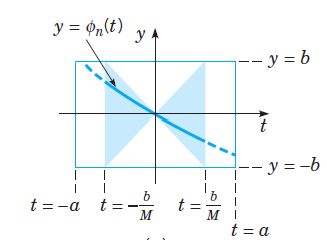
\includegraphics[width=100pt]{wedge.png}
            \end{center}
            which is for $|t| \leq b/M$.
        \item \textbf{Does the sequence ${\phi_n(t)}$ converge?}
            \newline \indent
            We can identify $\phi_n(t) = \phi_1(t) + [\phi_2(t) - \phi_1(t)] + [\phi_3(t) - \phi_2(t)] + \dots + [\phi_n(t) - \phi_{n-1}(t)]$ as the $n$th partial sum of the series
            \begin{equation*}
                \phi_1(t) + \sum_{k+1}^\infty [\phi_{k+1}(t) - \phi_k(t)]
            \end{equation*}
            The convergence of the sequence ${\phi_n(t)}$ is established by showing that this series converges. 
            \newline
            TODO: PROVE THIS USING PROBLEMS 15-18
            \newline
            We denote the limit function by $\phi$, so that
            \begin{equation*}
                \phi(t) = \lim_{n \rightarrow \infty} \phi_n(t)
            \end{equation*}
            
        \item \textbf{What are the properties of the limit function $\phi$?}
            \newline \indent
            We know that $\phi$ is continuous since the sequence ${\{phi_n}$converges in a certain manner, known as uniform convergence. We proof we used proves this as well. Now let us return to
            \begin{equation*}
                \phi_{n+1}(t) = \int_0^t f[s, \phi_n(s)] ds
            \end{equation*}
            Allowing $n$ to approach $\infty$ on both sides, we obtain
            \begin{equation*}
                \phi(t) = \lim_{n \rightarrow \infty} \int_0^t f[s, \phi_n(s)] ds
            \end{equation*}
            We can move the limit inside the integral since the sequence converges uniformly.
            \begin{equation*}
                \phi(t) = \int_0^t \lim_{n \rightarrow \infty} f[s, \phi_n(s)] ds
            \end{equation*}
            Then we take it inside the function
            \begin{equation*}
                \phi(t) = \int_0^t f[s, \lim_{n \rightarrow \infty} \phi_n(s)] ds
            \end{equation*}
            so
            \begin{equation*}
                \phi(t) = \int_0^t f[s, \phi(s)] ds
            \end{equation*}
            Moving the limit inside the function is saying that $f$ is continuous in its second variable, which is known. So this last equation shows that $\phi$ satisfies the integral equation so it is a solution for the initial value problem.
        \item \textbf{Are there other solutions of the integral equation besides $y = \phi(t)$?}
            \newline \indent
            Assume another solution $y = \psi(t)$. It can be shown that
            \begin{equation*}
                |\phi(t) - \psi(t)| \leq A\int_0^t |\phi(s) - \psi(s)| ds
            \end{equation*}
            TODO: Prove this using PROBLEM 19
            \newline
            for $0 \leq t \leq h$ and a suitable positive number $A$. It is now convenient to introduce $U$ as
            \begin{equation*}
                U(t) = \int_0^t |\phi(s) - \psi(s)| ds
            \end{equation*}
            \begin{align*}
                U(0) = 0 \\
                U(t) \geq 0, \quad \text{for } t \geq 0
            \end{align*}
            $U$ is differentiable, and $U'(t) = |\phi(t) - \psi(t)|$.
            \begin{equation*}
                U'(t) - AU(t) \leq 0 \text{ for } 0 \leq t \leq A/2
            \end{equation*}
            Multiplying by $e^{-At}$ gives
            \begin{equation*}
                [e^{-At}U(t)]' \leq 0  \text{ for } 0 \leq t \leq A/2
            \end{equation*}
            Then, by integration from 0 to $t$
            \begin{equation*}
                e^{-At}U(t) \leq 0  \text{ for } 0 \leq t \leq A/2
            \end{equation*}
            Hence $U(t) \leq 0$ for $0 \leq t \leq A/2$, but since $A$ is arbitrary $U(t) \leq 0$ for all positive $t$. Since $U(t) \geq 0$, $U(t) = 0$, so $U'(t) = 0$ and $\psi(t)= \phi(t)$. This proves there connot be two different solutions to one initial value problem for $t \geq 0$. A slight modification of this argument shows the same is true for $t \leq 0$.
    \end{enumerate}